\documentclass[conference,final]{IEEEtran}

\usepackage{graphicx}
\usepackage{epsfig}
\usepackage{subfigure}
\usepackage[hypertex]{hyperref}
\usepackage{subfigure}  
\usepackage{color}
% \usepackage{draftcopy}

\usepackage[small,it]{caption}

\usepackage{multirow}
\usepackage{ifpdf}

% \newcommand{\jha}[1]{\textcolor{red}{\bf Jha:} }
% \newcommand{\hartmut}[1]{\textcolor{blue}{\bf Hartmut} }
% \newcommand{\yaakoub}[1]{\textcolor{green}{\bf Yaakoub} }
% \newcommand{\ole}[1]{\textcolor{red}{\bf Ole} }

\newcommand{\jha}[0]{}
\newcommand{\hartmut}[0]{}
\newcommand{\yaakoub}[0]{}
\newcommand{\ole}[0]{}

\newcommand{\fixme}[1]{ { \bf{ ***FIXME: #1 }} }
\newcommand{\jhanote}[1]{ {\textcolor{red} { ***Jha: #1 }}}
%\newcommand{\jhanote}[0]{}
\newcommand{\jitter}[1]{{$\sigma(\alpha)$}}

\newif\ifpdf
\ifx\pdfoutput\undefined
  \pdffalse
\else
  \ifnum\pdfoutput=1
    \pdftrue
  \else
    \pdffalse
  \fi
\fi

\ifpdf
\DeclareGraphicsExtensions{.pdf, .jpg}
\else
\DeclareGraphicsExtensions{.eps}
\fi


\begin{document}


\title{\large Design and Implementation of Network Performance Aware
  Applications Using SAGA and Cactus}

\author{\authorblockN{Shantenu Jha\authorrefmark{1}\authorrefmark{2},
    Hartmut Kaiser~\authorrefmark{1}, Yaakoub El
    Khamra\authorrefmark{1}, Ole Weidner\authorrefmark{1}}
  \authorblockA{\authorrefmark{1} Center for Computation and
    Technology, Louisiana State University, Baton Rouge, 70803}
  \authorblockA{\authorrefmark{2} Department of Computer Science,
    Louisiana State University, Baton Rouge, 70803} }

\maketitle

\begin{abstract}
  This paper demonstrates the use of appropriate programming
  abstractions -- SAGA and Cactus -- that facilitate the development
  of applications for distributed infrastructure.  SAGA provides a
  high-level programming interface to Grid-functionality; Cactus is an
  extensible, component based framework for scientific applications.
  We show how SAGA can be integrated with Cactus to develop simple,
  useful and easily extensible applications that can be deployed on a
  wide variety of distributed infrastructure, independent of the
  details of the resources. Our model application can gather and
  analyze network performance data and migrate across heterogeneous
  resources.  We outline the architecture of our application and
  discuss how it imparts important features required of eScience
  applications.  As a proof-of-concept, we present details of the
  successful deployment of our application over distinct and
  heterogeneous Grids and present the network performance data
  gathered.  We also discuss several interesting use cases for such an
  application -- which can be used either as stand-alone network
  diagnostic agent, or in conjunction with more complex scientific
  applications.
\end{abstract}

\begin{keywords}
  eScience Application, Middleware Inter-operation, Distributed
  Infrastructure Deployment, Distributed Application Programming,
  Cactus, Performance, SAGA, Lightpaths
\end{keywords}

\section{Introduction}

A critical component in the original definition of e-Science by John
Taylor, is the notion of an e-Infrastructure that will enable novel
and different research~\cite{hey03}. Conversely, e-Science
applications must be able to utilize e-Infrastructure -- whether
sophisticated services, or the next generation networks or customized
supercomputers -- to perform better, faster and different domain
specific research~\cite{hey04, hey05}. But can applications be easily
developed to exploit e-Infrastructure in ways that were not possible
before and thus be used to perform ``novel'' (better, faster and
different) research?  Such e-Infrastructure, almost by definition, is
dynamic -- changing in both qualitative and quantitative aspects.
Thus the question is how can we design and develop e-Science
applications, that on the one hand are not limited by the complexity
of e-Infrastructure, while on the other hand are immune to the
evolving nature of such infrastructure?

% be developed but also such that they are immune to the evolving nature
% of such infrastructure?

There are several plausible solutions to the above conundrum, but
arguably one of the most significant is the need for programming
abstractions that enable the easy creation of applications that are
independent of the details of the underlying infrastructure.  In other
words, the ability to develop novel applications that can be
explicitly created and programmed to harness features provided by the
e-infrastructure is critical.  It is generally accepted that there
exist rather limited support for the development of such distributed
applications, in particular high-level programming abstractions that
could facilitate the development of such applications are missing.

SAGA is a simple high-level programming abstraction that provides some
of these requirements.  It has been compared to the
MPI~\cite{mpiforum_url} for Grid Programming, in that SAGA provides
simplified method calls at the right level of abstraction for the most
commonly required Grid-functionality.  In addition to being simple, an
additional critical feature of SAGA is that it is on the road to
becoming a community standard, thus strengthening the analogy with
MPI.  SAGA in conjunction with Cactus -- which is a component based
framework that enables the creation of modular parallel and
distributed applications -- provides an appropriately layered
abstraction that enables the creation of middleware independent
applications.  The SAGA-Cactus approach is consistent with the central
tenet of an effective e-Infrastructure as outlined in
Ref.~\cite{hey05}: the e-Science community should focus on
building higher-level services specific to the application domain,
while responsibility for the design of the basic components of a
reliable underlying infrastructure is left to the IT industry.

% \jhanote{In Introduction, we will need a paragraph about SAGA. Then
%   SAGA \& Cactus coupling.}

In this paper, we report on the development of a network-centric
application using SAGA and Cactus, that is capable of acquiring
application-specific network characteristic data. This data can be
analyzed by the application to dynamically determine the optimal set
of resources to utilize, and having done so is capable of migrating to
the optimal set of resources.  This application can be deployed on any
resource independent of the middleware stack. All that is required is
support for SAGA {\it adaptors} -- the middleware specific glue layer
that enables the middleware to parse the appropriate SAGA function
calls and implement the correct functionality.  As SAGA becomes a
standard~\cite{saga-uc, saga-req, saga-core} there will be increased
willingness on the part of middleware developers and resource
providers to provide these adaptors to the application community.
Additionally, as the deployment of SAGA and required adaptors becomes
wider (pervasive) and deeper (greater functionality), there is an
increased incentive for application developers to use SAGA.

% consists of a exemplary distributed simulation that uses the added
% SAGA functionality to dynamically determine its ideal migration
% target based on ad-hoc and statistical network characteristics and
% to migrate itself in a heterogeneous Grid environment.

%\noindent 
%Before presenting an outline of the paper, ni
The highlights of this paper are:

%\noindent 
{\it Demonstrate the usefulness of SAGA for Grid application
  development:} SAGA provides a high-level programming interface to
Grid functionality, and thus presents arguably, for the first time
ever, the ability to develop complete and sophisticated applications
using simple Grid function calls.  This paper demonstrates the utility
of SAGA for creating applications that can perform across dynamic and
heterogeneous infrastructure.

%\noindent 
{\it Integrate SAGA and Cactus:} Cactus has a proven track
record of enabling high-performance application with novel
functionality~\cite{Cactus_GordonBell, Sidney_Fernbach}.  Thus it is
natural that we try to utilize the many important and interesting
features that it provides for developing novel distributed e-Science
applications. As alluded to, we do so by interfacing SAGA with Cactus
and thus are able to draw on the many advantages of using SAGA
function calls from within a Cactus application.  The result is the
first application that uses these two important application-level
abstraction(s) to create a truly distributed application.~\footnote{It
  is interesting to note that although we use the Cactus framework, in
  principle, Cactus can be swapped for any framework which provides
  similar levels of abstraction and functionality and which is
  consistent with the common component architecture.}

%\noindent 
{\it Utilize the advantages of proper programming abstractions:}
Although we focus on a specific application -- gathering network
characteristics for a Poisson Equation solver and migrating the
application -- thanks to the architecture and abstractions used,
similar functionality can be trivially incorporated in more
sophisticated and complex applications.

%\noindent 
{\it An effective e-Science application:} The application we
developed using SAGA and Cactus, although simple is a meaningful and
useful e-Science application.  We will establish this fact by
collecting and analyzing network performance characteristics across
heterogeneous infrastructure -- using SAGA function calls. In addition
to providing a core motivation, we will discuss several use cases that
can benefit from simple extensions and generalizations of the
application we develop.

% Application can run on different, developing and
% dynamic (ie.  changing) infrastructure - SAGA is one high level;
% Cactus is the level of abstraction. 
%\item Push the production grade deployment of SAGA on LONI (private
%  motivation) \jhanote{this is a private motivation}

The outline of the paper is as follows: In the next section we
describe the details of the components that are used to develop the
application that we have developed to monitor network characteristics
using SAGA and Cactus, and provide both the motivation for the
specific application as well as several use case(s) for the
(generalized version of the) application. This section provides
details of the algorithm that the application uses to spawn itself
onto a set of resources.  In Section III, we discuss the architecture
of the application. Section IV provides a brief description of the
heterogeneous Infrastructure (test-bed) that we use to deploy this
application. Finally we present the data collected by this application
and some simple analysis in Section V.

\section{Application: Description and Motivation}

\subsection{Application Outline}

The aim of our model application is to show the potential and ease of
use of a SAGA-enabled Cactus framework application. Our application
consists of a exemplary distributed simulation that uses the added
SAGA functionality to dynamically determine its ideal migration target
based on ad-hoc and statistical network characteristics and to migrate
itself in a heterogeneous Grid environment.  Although this a model
application it can be easily adapted to more complex scientific
applications.  Furthermore, our model application can be used as an
autonomous benchmarking agent for Grid resources. In this section we
briefly describe SAGA and the Cactus framework and discuss our
motivation to use SAGA to incorporate high-level Grid functionality
into Cactus.

%Aim of the current application is to be able to gather network
%performance information and make it available to the ``remainder'' of
%the application, so as to enable the application to make decisions
%about the its progress.  The network characteristic gathering operates
%as regular scientific application independent of the core functionaliy
%of the application.

\begin{figure}
\begin{center}
\includegraphics[scale=0.30]{./figures/figure_00}
\end{center}
\caption{The model application is a distributed simulation that uses ad-hoc network measurement and collected network statistics to determine its ideal migration target within a heterogeneous Grid environment. }
\label{fig:algo}
\end{figure}

%Outline of the application algorithm. The application
%determines the resources -- usually user defined -- that it should
%migrate on to, spawns a copy of itself onto that resource,
%establishes a connection with the original host to monitor network
%performance, before spawning further.  This is a dynamic,
%network-aware, application...}

\subsubsection{SAGA}

The Simple API for Grid Applications (SAGA) is an API standardization
effort within the Open Grid Forum (OGF)~\cite{ogf_web} -- an
international committee that coordinates the standardization of Grid
middleware and architectures. SAGA provides a simple, POSIX-style API
to the most common Grid functions at a sufficiently high-level of
abstraction so as to be able to be independent of the diverse and
dynamic Grid environments.  The SAGA specification defines interfaces
for the most common Grid-programming functions grouped as a set of
functional packages.  Version 1.0~\cite{saga-core} of the
specification has been submitted to the OGF editorial pipeline and is
currently under review.  It defines the following packages:

\begin{itemize}
\item File package - provides methods for accessing local and remote
  filesystems, browsing directories, moving, copying, and deleting
  files, setting access permissions, as well as zero-copy reading and
  writing
\item Replica package - provides methods for replica management such
  as browsing logical filesystems, moving, copying, deleting logical
  entries, adding and removing physical files from a logical file
  entry, and search logical files based on attribute sets.
\item Job package - provides methods for describing, submitting,
  monitoring, and controlling local and remote jobs. Many parts of
  this package were derived from the largely adopted
  DRMAA~\cite{drmaa_url} specification.
\item Stream package - provides methods for authenticated local and
  remote socket connections with hooks to support authorization and
  encryption schemes.
\item RPC package - is an implementation of the GGF GridRPC
  API~\cite{gridrpc_url} definition and provides methods for unified
  remote procedure calls.
\end{itemize}

The two critical aspects of SAGA are its {\it simplicity} of use and the
fact that it is well on the road to becoming a community {\it standard}.
It is important to note, that these two properties are 
provide the added value of using SAGA for Grid application development.
Simplicity arises from being able to limit the scope to only the most
common and important grid-functionality required by applications.
There a major advantages arising from its simplicity and imminent
standardization.  Standardization represents the fact that the
interface is derived from a wide-range of applications using a
collaborative approach and the output of which is endorsed by the
broader community.

For our current work we incorporated the SAGA C++ reference
implementation~\cite{saga_web} into the Cactus Code Framework to
provide the needed Grid programming functionality. The SAGA C++
reference implementation is being developed in close conjunction with
the OGF standard. Furthermore, our C++ implementation is the basis 
for the development of the SAGA C++ language binding specification 
currently going on at OGF, ensuring
full conformance with the main SAGA API specification.
It The current 0.6 release implements all
functional packages described above as well as an additional
Advert-service package which will most-likely be incorporated into a
future version of the OGF standard.  The available Grid-middleware
bindings (adaptors) delivered with current 0.6 release of the SAGA C++
reference implementation comprise a complete set of local adaptors, an
SQlite3 and PostgreSQL advert-service adaptor, and Globus preWS
adaptors for the file (GridFTP) and job (GRAM2) package.

% As is obvious (and the primary intent) SAGA can be used not only for
% distributed application development, but also be used at different
% levels -- service deployment and tool-development, in addition to
% application.

% SAGA can be used at  different levels of the spectrum -- application
% development, service deployment and tool-development. One persons
% application can be another persons tool.  
%One persons application can be another persons tool.
% used for (i) tool development -- e.g. AHE etc., as well as (ii)
% infrastructure development -- testing and deployment of
% services...\jhanote{requires attention}\\

\subsubsection{The Cactus Code~\cite{cactus_web}}

Cactus~\cite{X0} is a framework for high performance scientific
computing designed for scientists and engineers to develop and run
codes for solving complex problems.  Developing code for high
performance parallel machines has many challenges including
scalability, efficiency (for computation, communication and
input/output), portability and flexibility. Frameworks such as Cactus
allow scientists and engineers to develop modules which can then be
used together with modules written by other researchers to solve
complex computational problems. The framework provides tools ranging
from basic computational building blocks to complete toolkits that can
be used to solve complex problems in astrophysics, computational fluid
dynamics or other disciplines.  Tools developed in the Cactus Code
framework run on a wide range of architectures including desktop PC's,
supercomputers and computational Grids. Cactus and its associated
toolkits are publicly available for download from the Cactus Code
website.

From an architectural standpoint, the Cactus Code framework consists
of a central part (the ``flesh") and code modules (``thorns").  The
flesh serves as a module manager, scheduling the routines of the
thorns and passing data between thorns.  Thorns perform tasks ranging
from setting up the computational grid, decomposing the computational
grid for parallel processing, providing boundary and initial
conditions, communication of data from one processor to another,
solving partial differential equations to input and output and
visualization streaming. There are code modules that provide
simulation control tools, such as the HTTPD thorn that sets up a web
server for the simulation and allows researchers to control a
simulation or view sample output from a web interface.  Thorns can
also provide custom developed scientific or engineering applications,
such as computational fluid dynamics or gravitational physics.

Features of Cactus which make it particularly suited to take advantage
of a Grid environment include its portability, architecture
independent checkpoint and restart capabilities, steering interface,
and a well designed interface in the flesh for providing information
about grid variables, scheduling, parameters and so on.

Cactus has been a driving application for many Grid computing
projects.  An early experiment in 2000 called the Cactus
Worm~\cite{X1} showed how any Cactus application could be autonomously
migrated around the resources of the eGrid in Europe simply by adding
a new thorn which used the Globus MDS, GRAM and GridFTP APIs to access
Grid capabilities. A later collaboration with the GRADS project added
dynamic capabilities for resource selection and contract
negotiation~\cite{X2}.  These experiences led to the EU GridLab
project which experimented with Cactus migration as a driving
scenario~\cite{X3}.

% developed a Grid Application Toolkit (GAT)
% which a generic API for developing dynamic Grid applications, and used
% Cactus migration as a driving scenario~\cite{X3}.

Cactus was also used for early experiments in metacomputing, showing
how incorporating adaptive techniques into the Cactus driver layer,
such as dynamic load balancing, configuration of ghostzones, and use
of data compression could lead to acceptable scaling for large MPI
applications across multiple supercomputers. This work was awarded the
Gordon Bell prize in 2001~\cite{Cactus_GordonBell}.

\subsubsection{Why SAGA and Cactus?} 

Because of the modular structure of Cactus, any functionality provided
by a specific thorn is immediately available to any of the other
thorns in the configuration. For this reason we implemented a set of
new Cactus thorns providing an extensible set of functions allowing
the collection of netperf~\cite{netperf_web} based network performance
metrics. Additionally, the extensible nature of this set of thorns
permits additional metrics for any Cactus based application in the
future.  To integrate SAGA functionality into Cactus, a SAGA thorn was
developed that provides the basic SAGA installation information
(header files, libraries etc.)  to the thorns that require SAGA
capabilities.  SAGA provides different packages with a consistent and
uniform flavor, thus implementing thorns that have different
functionality (performance measurement and migrate thorns) using
different SAGA packages is preferable. Last but not least, using SAGA
and Cactus enables applications to specify and customize the network
performance characteristics that it needs; as we shall see later, the
ability to do so is a very useful feature.

\subsection{Motivation: Automated Checkpoint and Transfer of
  Applications:}

Cactus black hole runs can last many days while queues typically last
much less than one day. Hence a mechanism to automatically migrate a
simulation to another machine is useful. With changing resource
requirements during a simulation (as is the case with adaptive mesh
refinement) a mechanism which can take advantage of faster, cheaper or
more powerful machines is even more advantageous than simple
migration. As the primary Cactus simulation starts, it progresses
through the schedule of the routines in the configuration. One of
these routines regularly checks for the time left for the simulation
in the queue. Once that time is near a certain limit, usually a value
set by the user, a checkpoint of the simulation is forced and the
simulation termination routines are called. Checkpoint files can vary
in size from a few Gigabytes to a few TeraBytes and generally depend
on the size of the problem being solved. Blackhole Cactus simulations
run on up to thousands of processors and checkpoint to around 500
MegaBytes per processor ~\cite{Cactus_CCTTR} ~\cite{Cactus_Kamil06a}
~\cite{Cactus_Shalf05a}. With many terabytes of data that need to be
transferred, the knowledge of which resources can be readied first
will be important.

\subsection{Additional Use Cases}

We present three different usage scenarios; the first two represent
classes of application, while the third is related to the specific
case of remote visualization on optical lightpaths. We illustrate how
all three use cases can benefit greatly from our model applications or
minor variants thereof.

\subsubsection{Tightly-Coupled Applications}

We pose the following questions: If a tightly-coupled application, say
a distributed MPI code, had N potential resources to chose from, which
M should it choose based upon network performance connecting those M
resources?  As a distributed MPI applications, requires all-to-all
communication, if we choose M out of N resources, then there are $N!
\over M! (N-M)!$ possible combinations.  Which of these combinations
will have the best network performance and thus how to choose the best
M out of N resources~\cite{clade06}.  This is a problem that has been
encountered -- admittedly so far with small values of M and N, but
soon with M and N sufficiently large that simple (non-scalable)
solutions adopted so far (e.g., phoning system administrators) will not
work.

Given a fixed partition scheme, the general problem of how to
distribute an application over M resources is a non-trivial one.
There are potentially two distinct, orthogonal issues that need to be
considered: choosing resources that provide optimal scheduling versus
optimal distribution (network performance).  It is possible that the M
resources to choose are not necessarily the optimal M to choose from a
scheduling perspective, i.e., it is plausible that they have very
different queue load factors, or one or more of the M resources have
the longest wait times.  Resolving this coupled problem is not within
scope of this paper - it requires extension to the information
services that SAGA provides currently, so as to interact additionally
with something like the Network Weather
Service~\cite{wolski_cluster05, wolski_acm03, wolski_ccgrid02}.
But assuming that the M resources are
computationally equal, the problem then becomes an issue of how to
partition the problem such that communication is optimal.~\footnote{We
  are not interested in the general decomposition problem; as it is
  beyond the scope of this paper and we believe difficult to
  ``generalize'' to a range of applications; we will be concerned with
  the reduced problem, where the problem of interest is which M
  resources to choose such that the collective network performance is
  best.}  As alluded to, the general formulation of the problems
involves all-to-all communication, i.e., a fully-connected graph.
Specific implementations however, could lead to graphs with less
edges.  Also, communication might require symmetrical or asymmetrical
data transfer, i.e. not equally weighted edges.  Either way, the
ability to solve for an optimal configuration (based upon a fixed
partition scheme) is trivially solved by a thorn that can is capable
of implementing algorithms for flow optimization on graphs, i.e.
min-cut/max-flow~\cite{mincut-maxflow}.

Having determined which M resources to use, the way forward could be
using a Grid co-allocator such as HARC~\cite{harc_url}; that is,
having identified the best M resources from a network performance
perspective, we leave the co-scheduling of these M resources to HARC
which is an implementation of Paxos (two-phase) Commit Algorithm. We
will report on the interfacing of HARC with SAGA in the future.

\subsubsection{Loosely Coupled Applications}

Having focused on computationally-intensive applications for the
tightly-coupled applications, we will take the opportunity to discuss
data-centric examples for loosely coupled application.  Specifically
we will discuss data scheduling and placement jobs.

Stork~\cite{stork_url, kosar_scpe05} is a specialized scheduler for
data placement activities in heterogeneous environments.  It elevates
data placement activities to "first class citizens" on the Grid just
like the computational jobs by enabling such data placement jobs to be
queued, scheduled, monitored, managed, and even check-pointed.
Importantly, it ensures that they complete successfully and without
any human interaction.

When performing point-to-point transfers, Stork considers how to best
tune-up the parameters of the underlying protocol it is using. For
example, parameter values can change from protocol to protocol, i.e.
for GridFTP they are: number of parallel streams, TCP buffer size and
I/O block size.  Stork currently uses existing external network
monitoring tools to estimate these numbers for any given transfer.
The PerfMatrix thorn can be easily generalized to permit
experimentation with various protocols (e.g., TCP vs UDP vs UDT,
GridFTP parameters) and parameters associated with these transport
protocols.  But a crucial feature of Stork is that it does not have an
internal monitoring system that would enable it to determine network
characteristic and thus make the network performance-based decisions
that are most meaningful for the application at hand. Thus a logical
next step is to create an interface such that Stork can trivially
query and determine the network characteristics that it needs.  In
other words our model application can be used by Stork to make
decisions about which resources to use for data placement.

%\jhanote{failure recovery, dynamical optimization, related work}
% \jhanote{NWS programmatic interface in the short run; develop
%   Information Service Interface in the medium to long term}

% \jhanote{Need to have measurement over both lightpath and regular
%   network(s).  This probably means performance matrix probably needs
%   all the elements (as $P_{ij} \neq P_{ji}$)}

\subsubsection{Distributed Visualization:} 

The traditional visualization pipeline is: data source (which could be
a computational simulation) feeds into a renderer which inputs
into a display.  Remote visualization could have one or all aspects of the
pipeline located remotely. 

It is not difficult to see that remote visualization -- whether one
large rendering problem is broken up and distributed or several
``computational sources'' feed one single renderer -- is sensitive to
network performance.  Thus simple queries like, which M computational
resources have the same (best?) network characteristics to the
renderer?

Arguably the most common class of applications utilizing lightpaths
are remote visualization applications
~\cite{Lightpath_web1}. %~\cite{Lightpath_web2}
Even though the QoS lightpaths might be specified upfront, when
combining lightpaths, the end-to-end performance is often different
from single point-to-point theoretical performance; thus the
appropriate choice of the resources is useful.

Ref.~\cite{spice_escience06} showed how the performance of
high-performance realtime interactive applications is sensitive to
network characteristics.  When the transfer rate requirements are
relatively low, Ref.~\cite{spice_escience06} detailed how network
latency and jitter can influence the performance of high-end
simulations. Our application can be trivially generalized to acquire
latency and jitter statistics and thus enable applications to make the
decision about which machines to use for remote visualization and
interactivity.

\section{Application Implementation and Control Flow} 


\begin{figure}
 \begin{center}
 \includegraphics[scale=0.30]{./figures/figure_02}
\end{center}
\caption{The components of the application. The Cactus framework orchestrates the \textit{WaveToy} thorn as an example for a distributed calculation, the \textit{NetPerf} thorn for network performance measurement, and the \textit{SAGA Migration} thorn for replication and migration. The \textit{Advert DB}
stores and archives the measurement results. Note that the application runs under the control of a \textit{Resource Manager (RM)} using SAGA's job management package.}
 \label{fig:arch}
 \end{figure}

%  \jhanote{How does the SAGA migrate thorn send performance information
%    to the Advert DB?  Shouldn't this come from the perfmatrix thorn?}
%  \jhanote{Where does Wave Toy come in? Are we coupling this to the
%    wave toy?}  \jhanote{Why label the box as an RM Job? Something
%    better required?}  \jhanote{Would straight lines be more
%    appropriate than the current curvilinear lines?}


\subsection { Application Architecture} 
The general architecture of the model application is based on the
programming abstraction provided by the Cactus framework. A set of
thorns that provide specific functionality are orchestrated by the
Cactus flesh as depicted in Fig.~\ref{fig:arch}. The novelty in this
Cactus application is that the complete SAGA API is known by the
Cactus build and deployment system and therewith transparently
accessible from within any thorn. With the SAGA functionality
available it was easy to implement Cactus thorns that can interact
with remote resource mangers (e.g. Globus GRAM2), copy, read, and
write files from and to remote locations (e.g. Globus GridFTP), and
access a remote PostgreSQL based advert service as logging and storage
facility. The properties and implementations of the individual thorns
are described in this section.

\subsubsection{WaveToy} The WaveToy thorn implements the simulation of
a 3D scalar field produced, for example by two orbiting sources.  This
is a simple thorn, but is part of a class of more complex systems,
including Einstein's field equations, Maxwell's or Navier-Stokes
equations.

\subsubsection{PerfMatrix} The PerfMatrix thorn takes care of the
intrinsic network performance measurement and persistent storage of
the results. Currently, the implementation uses
netperf~\cite{netperf_web} to measure unidirectional end-to-end
throughput. Netperf is implemented as a simple client-server model
consisting of two executables:
\begin{itemize}
\item{netserver: the measurement endpoint waiting for incoming connections}
\item{netperf: the initiator of a measurement connecting to a netserver endpoint}
\end{itemize}

The PerfMatrix algorithm uses a list of computational resources which
are potential migration targets for the application. After starting
up, the initial application spawns itself onto all available hosts.
\footnote{This approach is different from the original non-centralized
  spawning scheme shown in Fig.~\ref{fig:algo} The reason for our
  implementation using centralized spawning is the Globus Toolkit's
  (4.0.5) inability of full credential forwarding.} Once all jobs have
been launched, the original spawning application first establishes
netperf connections with all the spawned applications; this is
followed by the spawned applications establishing netperf connections
amongst each other, following the scheme shown in Fig.~\ref{fig:algo}.
The job spawning, control, and I/O redirection is done entirely using
SAGA's job management package.  Once a netperf process returns a
throughput result, the PerfMatrix thorn uses the SAGA advert-service
package to announce the result to a central PostgreSQL database which
is also used as a centralized logging facility. After all netperf
processes have finished and published their results, the database
contains a host-to-host throughput performance matrix along with a
timestamp which is available to other thorns as well as other
applications.

\subsubsection{Advert-service database} SAGA's advert-service package
describes a key-value based hierarchical attribute interface for
storing arbitrary information. The currently available adaptor is
capable to map these structures to an relational SQL schema and store
them in local (SQLite) and remote (PostgreSQL) RDBMS.

SAGA's advert-service offers a convenient way to simplify the
difficult task of centralized data collection and logging within
distributed applications. The advert structure consists of two
hierarchical trees: one for logging (containing the host name, a
timestamp, and the log message) and one for the throughput performance
matrix (containing a timestamp and the matrix itself). Since every
matrix is stored with a timestamp, every time the NetPerf thorn gets
triggered, an additional matrix is added to the advert-service which
leads to a growing stack of time-series data. This time-series can in
turn be analyzed by the SAGAMigrate thorn to determine if and where
to migrate.  Since all data stored in the advert-service can be
directly accessed using SAGA's high-level interface, it is easy to
browse the time-series data from other applications. A simple tool
that generates boxplots (Fig.~\ref{fig:boxplot}) from the performance
matrices is proof of the simplicity.

\subsubsection{SAGAMigrate} The SAGAMigrate thorn is a Cactus thorn
written in C++ that uses SAGA functions (for example file.copy and
job\_description.create\_job) to perform a simulation migration.
SAGAMigrate copies a restart parameter file and the checkpoint file(s)
from one machine to another (for example using the SAGA Globus
adaptors).

\begin{figure}
 \begin{center}
 \includegraphics[scale=0.30]{./figures/figure_01}
 \end{center}
 \caption{The algorithm used by the PerfMatrix thorn. Based on a list of resources, the application spawns itself, launches Netperf endpoints and measures the throughput of all possible connections. }
 \label{fig:algo}
 \end{figure}

 \subsection{Control Flow} 

% The application we have implemented makes use of the network
% characterisitics (gathered by the PerfMatrix thorn) the SAGAMigrate
% thorn, which allows a simulation to proceed by migrating to a
% different host once its allocated time is over.
% Our implementation of the simulation migration functionality is
%  activated.... at the simulation termination stage: the thorn

PerfMatrix measures the bandwidth between the primary simulation host
and a list of other candidate hosts. The results are stored in a
table accessible to other thorns in the configuration. The
SAGAMigrate thorn scans the table for the best candidate host to
migrate to. Once the best candidate host is selected, the SAGAMigrate
thorn copies the checkpoint and parameter files from the primary host
to the best candidate host and restarts the Cactus simulation to pick
up where it had left off on the primary host.

The current implementation has SAGAMigrate select the best host based
on the maximum bandwidth connectivity to that host. Our current
implementation uses SAGAMigrate parameters, variables that can be set
at runtime and are steerable, to set the network benchmark executable.
With steerable parameters, the user can decide at runtime what the
best metric is and set the appropriate benchmark parameters in
SAGAMigrate. With a more sophisticated performance metric the
selection algorithm would require revision beyond the current
``maximum bandwidth'' approach, for example measurements to be made,
by a query to the Network Weather Service ~\cite{NWS_web, bqp_url} or
a small application benchmark to estimate time to completion.

Another use of SAGAMigrate is to move simulation results from one
machine to another to run a different application. A typical scenario
would be a Cactus simulation migrating its results to another machine
and starting an analysis tool, a data mining tool or a visualization
application. With a fully parameterized interface to both application
and data, the current implementation of SAGAMigrate can perform basic
workflow staging across machines and applications.


%the PerfMatrix thorn behaves as a regular set of netperf end points.

\section{Infrastructure Used \& Deployment Details}

%{\bf SURAGrid, LONI and GumboGrid: Three distinct Grids?}
%\fixme{Need to describe if they are all Globus Grids?}

\subsection{Infrastructure}

We use two different Grids to deploy our application and collect data:
LONI (a State-wide Grid) and GumboGrid (a LSU campus wide
Grid).\footnote{We also deployed our application successfully on
  SURAGrid~\cite{suragrid_web} but were unable to get performance data
  due to {\it unusual} firewall issues.}

% SURAgrid is a USA wide consortium of about 60 organizations
% collaborating and combining resources to help bring Grid technology to
% the level of seamless, shared infrastructure. The vision for SURAgrid
% is to orchestrate access to a rich set of distributed capabilities in
% order to meet diverse users' needs. Capabilities to be cultivated
% include locally contributed resources, project-specific tools and
% environments, highly specialized or HPC access, and gateways to
% national and international cyberinfrastructure~\cite{suragrid_web}.
% Consequently, the SURAGrid is built of a highly heterogeneous Grid
% infrastructure.

The Louisiana Optical Network Initiative~\cite{LONI_web} (LONI) is the
result of the convergence of recent trends in computing: advances in
the seamless coupling of distributed and heterogeneous resources along
with remarkable advances in optical networking which now enables
networks to be first-class resources, i.e. schedulable and with a
given quality-of-service.  In addition to providing dedicated
lightpaths, ~\footnote{A lightpath is a direct network path from one
  computer to another for which a permanent or temporary connection of
  fiber-optic cables is configured without using routers. Traffic on a
  lightpath does not encounter any other traffic. It therefore reaches
  its destination without congestion or contention.}  LONI also
provides an anticipated 85 teraflops of computational capacity. It has
5 IBM Power5 575 AIX machines installed at various university campuses
in Louisiana, along with 6 Dell 5 teraflop Intel Linux machines housed
at 6 LONI member institutions, and 1 Dell 50 teraflop Intel Linux
machine (Queen Bee, currently ranked 23 on the Top 500 list). The
infrastructure provided by LONI -- dedicated lightpaths with powerful
machines at the endpoints -- opens the door for new applications with
interesting functionality and features.

% LONI is still in its initial developmental state,
% currently with only three active IBM p5 machineswhich are housed at:
% Louisiana Tech (bluedawg.loni.org) Tulane (ducky.loni.org) University
% of Louisiana, Lafayatte (zeke.loni.org) and the University of New
% Orleans (neptune.loni.org).

GumboGrid is a small campus-wide Grid built out of two development
Beowulf style clusters, each of these having 5 nodes.  Both clusters
are located at different locations on the LSU campus and, do not share
a special interconnection with each other.  Interestingly, in
measuring the network characteristics of the Grid resources used we
have a hybrid of best-effort networks and dedicated lightpaths.
Traffic between the LONI machines is over dedicated lightpaths, while
traffic GumboGrid machines is over best-effort networks as is that
traffic between the GumboGrid machines and between LONI.

% {\it Negative point here is: if one machine is used to measure network
%   performance along two network paths simultaneously, these
%   measurements are not independent anymore, since these may use the
%   same network interface at the same time.}

% LONI (Louisiana Optical Network Initiative) is a fiber optics network
% infrastructure connecting the supercomputers at Louisiana's major
% research universities

\subsection{Deployment}
The deployment of applications across a pool of heterogeneous machines belonging to different Grids and organizations can be a difficult task. Different versions and availability of libraries and compilers makes every single machine a unique environment. Although it is technically possible to stage-in all required applications and libraries and even to compile the application sources on the fly using SAGA, we decided to deploy pre-build binaries on all machines since this exercise is not part of this work's focus.

Since both, the Cactus framework and SAGA aim to be as platform-independent as possible, the deployment process was rather straightforward - the only noteworthy problems occurred during the initial attempt to build SAGA on LONI's 64bit AIX 5L nodes. The problems were mainly caused by the IBM's xlC++ compiler's inability to handle C++ partial template instantiation, a broken AIX pthread implementation and the absence of usable debugging tools. Although the deployment process on AIX was very time consuming it eventually led to a vastly improved SAGA build system and a more conservative use of C++ template mechanisms which ensures the support of other non-standard compilers.

\section{Results and Discussion}

\begin{figure}
\begin{center}
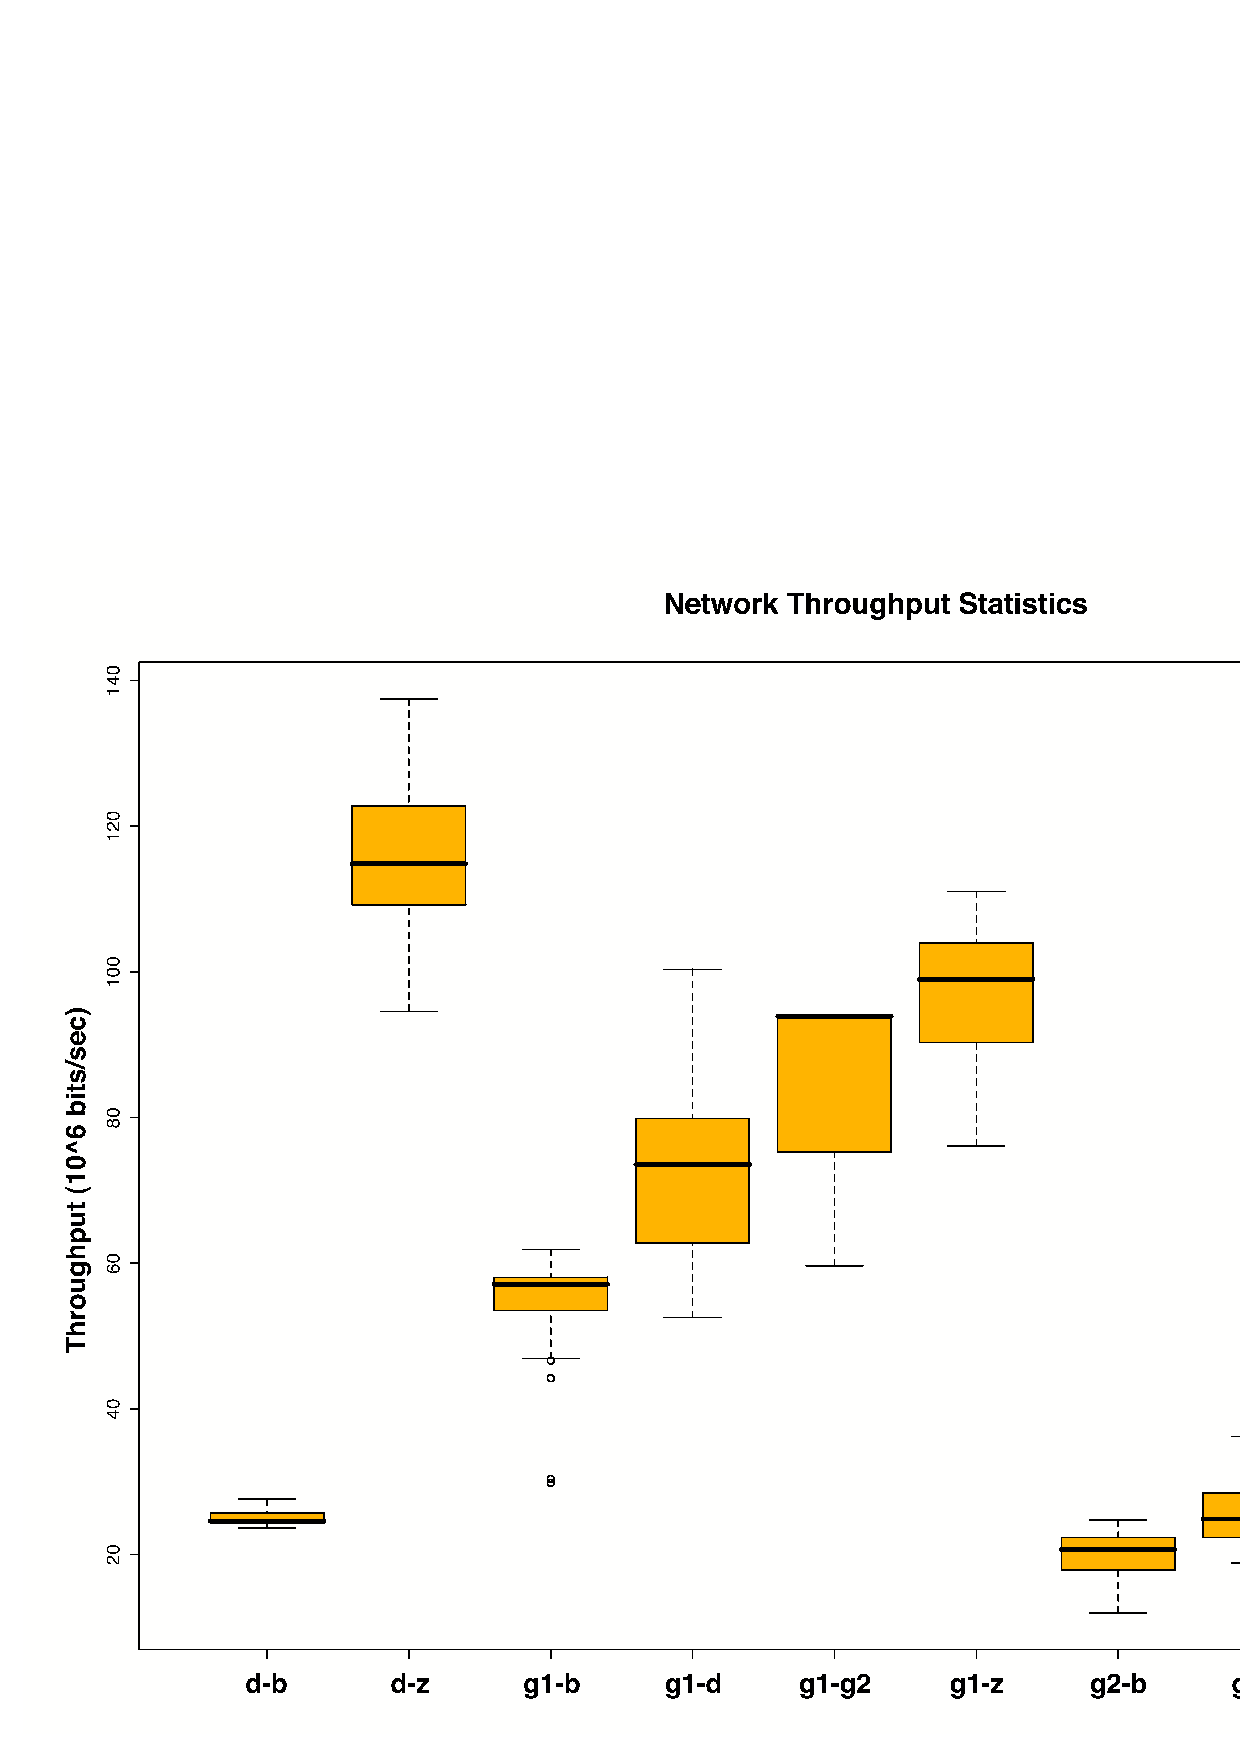
\includegraphics[scale=0.30]{./figures/figure_04}
\end{center}
\caption{Network throughput statistics extracted from the advert-service database after running the NetPerf thorn for 12 hours in 10 min. intervals. The letters on the X-axis stand for: d(ucky.loni.org), b(luedawg.loni.org), z(eke.loni.org), g1 (gg101.cct.lsu.edu), g2 (gg201.cct.lsu.edu)}
\label{fig:boxplot}
\end{figure}

The SAGAMigrate thorn from WaveToyCXX application parsed data gathered
and based upon that was able to determine which machine to migrate
too. The data gathered over twelve hours at a sampling interval of ten
minutes between the five different resources is shown (using the
Box-and-Whitney format) in Fig~\ref{fig:boxplot}.  As the data
collected shows, our simple application can now serve as a stand-alone
diagnostic tool for networks maintenance and monitoring.  Simple
extensions to the features of the network monitoring thorns,
%endow it with features required to 
will make it a full-fledged network diagnostic tool to meet the needs
of LONI for the different use cases discussed in Section II C.

The PerfMatrix thorn provides the capability to use either Time Series
(historical) data or instantaneous real-time data for analysis.  The
ability to collect and analyze both sets is important: for relatively
short-lived transactions real-time data is the more useful information
in order to make placement decisions. For long-time transfers, say of
the order of many terabytes or petabytes, the historical activity is
more relevant, especially if network characteristics are bursty

It is important to mention that similar to solving the computational
job-placement problems (which as alluded to, is a combination of the
job-scheduling and transfer), solving the generalized data-placement
problem -- which in turn is a composition of data-scheduling and
transfer -- is non-trivial.  Current network tests and
parameterizations implemented in the PerfMatrix thorn are simple and,
there are no attempts at dynamical optimization. Advanced modeling
techniques such as Markov-State transition models and others derived
from Queuing Theory are required to solve the complete placement
problem -- for both the data and computational cases as discussed
Sections II C.  It is important to note that whatever the underlying
prediction mechanism or model, it can be encapsulated within a thorn
and used by any application. Arguably for the first time ever, it is
possible to interface different performance and prediction model
directly with the application, and not at the middleware level or
external has been made possible.

A critical feature of this application which arise from using the
correct abstractions (SAGA and Cactus) is {\it the ability to separate
  the computational logic from the distributed logic.}  For example,
jobs on different resources, establish connections pair wise and
collect information which is published to an advert service through
SAGA's job-management package, whilst the PerfMatrix thorn remains
independent of the distributed aspects of the set of netperf
end-points.  Additionally, beyond compiling the application code on
the other resources, there is no need for the application to know
about the details of the middleware/platform of the remote resources.

\section{Future Work and Conclusion}

We have demonstrated that with the use of high-level grid primitives
and abstraction layers (SAGA and Cactus), development of grid aware
applications is made much easier. Integrating SAGA in Cactus allows
developers to focus on computational logic and algorithms and not have
to worry about the details of implementing the grid functionality. To
do this without these appropriately abstracted layers is difficult if
not impossible.  We developed PerfMatrix and SAGAMigrate thorns.  The
former acquires and analyzes application-specific network
characteristics; the latter migrates applications respectively.  We
have also demonstrated how these thorns act as service applications,
which can be easily interfaced with legacy applications and handle a
wide range of performance requirements. As discussed in Section II,
PerfMatrix and SAGAMigrate thorns can be easily extended to accommodate
the requirements of a wide range of applications -- tightly-coupled,
loosely-coupled and remote-visualization.

In fact, efforts are now underway to extend and interface an
appropriate PerfMatrix thorn for distributed MPI
applications~\cite{clade06}.  We have also begun work on creating the
relevant PerfMatrix thorn, to determine an optimal resource
configuration for remote visualization applications on LONI.

Our experience should serve as useful input to the community --
resource providers and middleware developer - to support the
development and deployment of SAGA Adaptors.  We created a single set
of Globus adaptors and deployed them on distinct Grids. Our
application successfully utilized these adaptors, without any further
customization, which goes to show that the widespread availability of
SAGA adaptors is an important step towards the creation of distributed
applications that can be universally deployed (i.e.  independent of
the details of the resource's middleware and configuration detail). We
hope to motivate both middleware developers and resource providers
(such as TeraGrid, EGEE, etc.) to subscribe to the SAGA philosophy and
thereby contribute to the development of SAGA adaptors for their
middleware stack as well as deploying these SAGA adaptors.

We also discussed how the deployment of this model application across
two distinct Grids was trivial as it only required the deployment of
of the appropriate SAGA adaptors.  Thus developing both applications
and tools using SAGA is an effective mechanism for ensuring
inter-operability across different middleware distributions -- even at
the application level -- something that is arguably missing in current
Grid Interoperation efforts~\cite{gin_paper}

% \jhanote{Reference GIN paper} Deployment is made easier because the
% same interface can be used universally and the complexity of making
% those function calls work/implemented has now been moved into the
% adaptor-middleware interface, i.e., in the territory away from the
% application domain!

There are many applications that need to use federated
Grids~\cite{clade06, gin_paper}.  Utilizing SAGA to develop, or at
least provide Grid-functionality is a useful strategy. Therefore, if
the development and deployment of applications across federated grids
is to be facilitated, SAGA adaptor activity -- development and
deployment, needs to be self-sustaining and thus requires explicit
support, from both the middleware developers and resource providers.

The success of e-Science critically depends upon the availability of
e-Infrastructure.  But the promise of e-Science will be hollow without
delivery of the applications and application-enabling paradigms and
technology that can effectively utilize this new infrastructure. We
believe SAGA is an important first step in this direction.

\section{Acknowledgements}

This work has been made possible thanks to the internal resources of
the Center for Computation \& Technology (CCT) at Louisiana State
University.  Important funding for SAGA specification and development
has been provided by the UK EPSRC grant number GR/D0766171/1 (via
OMII).  We would like to acknowledge the support of the OGF SAGA
Research Group for their work towards developing the SAGA
specification (in particular Andre Merzky), as well as the Cactus
team.  Additionally, we would like to acknowledge help from the LONI
support team and CyberInfrastructure Develompent group (CyD) in the
CCT.  We would like to thank Gabrielle Allen for useful input on the
manuscript. Finally, SJ acknowledges the e-Science Institute, Edinburgh for
supporting the theme, ``Distributed Programming Abstractions''.

\bibliographystyle{IEEEtran}
\bibliography{saga_cactus_escience}

\end{document}

% \jhanote{Two main strands of conclusion: First is the demonstrated
%   ability to develop interesting and novel eScience applications using
%   appropriate abstractions such as SAGA and Cactus.  Second is the
%   specific model application that we have created as proof-of-concept,
%   which although elementary and currently limited, is easily
%   extensible and thus widely usable/required -- as demonstrated in the
%   Use Cases}


% This is a lightweight application, that can be customized to meet
% specific application-level needs. One could in principle modify the
% code to place sensors inside the code which provide data gathering,
% load-balancing etc.. Our approach is different in that this an
% external agent that enables the core application to remain unchanged.
% ``service application''.

% This is an elementary application, but one that establishes the
% advantages of designing Grid-aware applications (or at least
% Grid-functionality of applications) using SAGA.  To do this without
% these appropriately abstracted layers is difficult if not impossible.
% Additionally this ``service application'' can be (i) easily interfaced
% with other legacy applications (as it requires only a (a) SAGA Thorn
% (b) performance thorn), (ii) a wide range of specific performance
% requirements can be accommodated within this framework. 
% Discuss for example, how it is trivial to use this application for the
% scenario in Use Cases 
%...\jhanote{which use case?}

% Development is made easier through the availability of high-level, Grid-primitives. 
% Thus the focus can be on the computational logic and algorithm and not the
% details of implementing the Grid-functionality i.e., marshalling distributed
% resources.
